
\documentclass[12pt,a4paper]{article} 

\usepackage{float,times,graphicx,mathtools}
\usepackage{amsmath}
\usepackage{amsfonts}
\usepackage{amssymb}
\usepackage{latexsym}
\usepackage{epsfig}
\usepackage{graphicx}
\usepackage{caption}
\usepackage{subcaption}
\usepackage{color}
\usepackage{pdfpages}
\usepackage{natbib}
\usepackage[space]{grffile}
\usepackage{wrapfig}
\usepackage{subcaption}
\usepackage{url}
\usepackage{bbm}
\usepackage{tikzsymbols}

\DeclareMathOperator{\logit}{logit}
\DeclareMathOperator{\tr}{tr}
\bibpunct[, ]{(}{)}{;}{a}{,}{,}
\graphicspath{{../}}  
\addtolength{\oddsidemargin}{-1in}
	\addtolength{\evensidemargin}{-1in}
	\addtolength{\textwidth}{1.75in}
	\addtolength{\topmargin}{-1.3in}
	\addtolength{\textheight}{2in}
\date{\vspace{-5ex}}
\begin{document}


\begin{itemize}
\item Changed how I calculate $s_x$ for the second last age group
\item Changed how to calculate $_0q_5$ that was previously slightly off
\item Given the hypervariance for $h$ a tighter prior and hypervariance for	$k$ a more diffused prior, if I loosen the prior on $h$ hypervariance I get crazy estimates again
\item Switched to using UNPD census counts instead of WPP population estimates (but using 1960 WPP estimates as baseline)
 \begin{itemize}
 \item[--] use a separate hypervariance for the baseline population?
 \end{itemize}
\item Tried fitting to only 0 - 50+, 0 - 50, 5 - 50+, 5 - 50, with different combinations of MVN, AR, ARIMA on $h$ and $k$,estimated $h$ are sill lower than IGME estimates
\item Tried using AR around common mean for $k$ and AR around 0 for $k$, estimated precision for $k$ varies such that in both case are around 2.7
\item Tried fitting to just the DHS data, the IGME priors are effective
\item Results below shown are fitted to 0-85+ Burkina Faso females
\begin{itemize}
  \item[--] Estimated $\rho$ for $h$ and $k$ are very close to 1, hence the almost parallel estimate $h$ to the IGME estimates
  \item[--] Wiggly estimated $f_x$ (but the magnitude is small?)
	\item[--] Estimated migration proportion insensible at the oldest age groups
	\item[--] Estimated $_{45}q_{15}$ are higher than WPP estimates most of the time
  \item[--] Currently estimating logit($\rho$), i.e. $\rho$ can only be within $(0,1)$, should I scale it to $(-1,1)$?
	\item[--] Fitting too closely to population data?
	\item[--] Estimated 0-4 population seems to be consistently higher than the raw data and parallel?
\end{itemize}
\end{itemize}

\newpage
\begin{figure}[H]
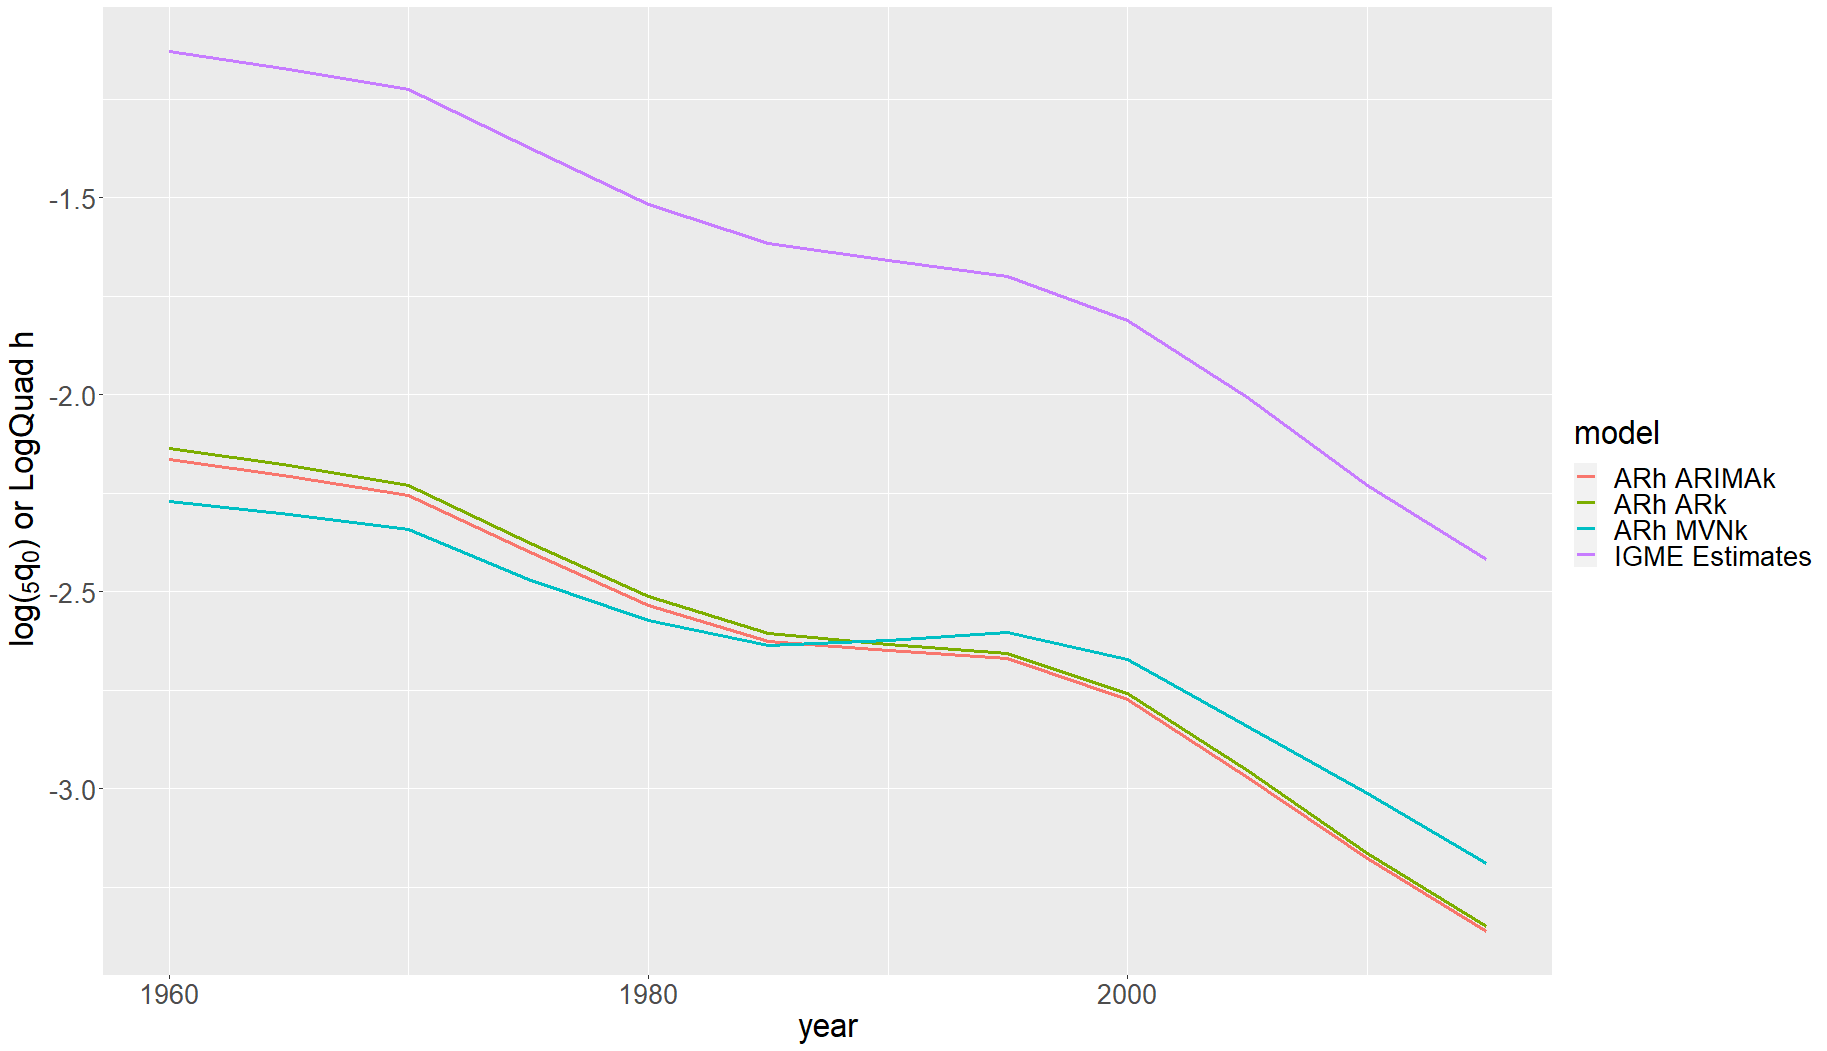
\includegraphics[width = \linewidth]{Burkina Faso/5/h.jpg}
\caption{Estimated $h$}
\end{figure}
\begin{figure}[H]
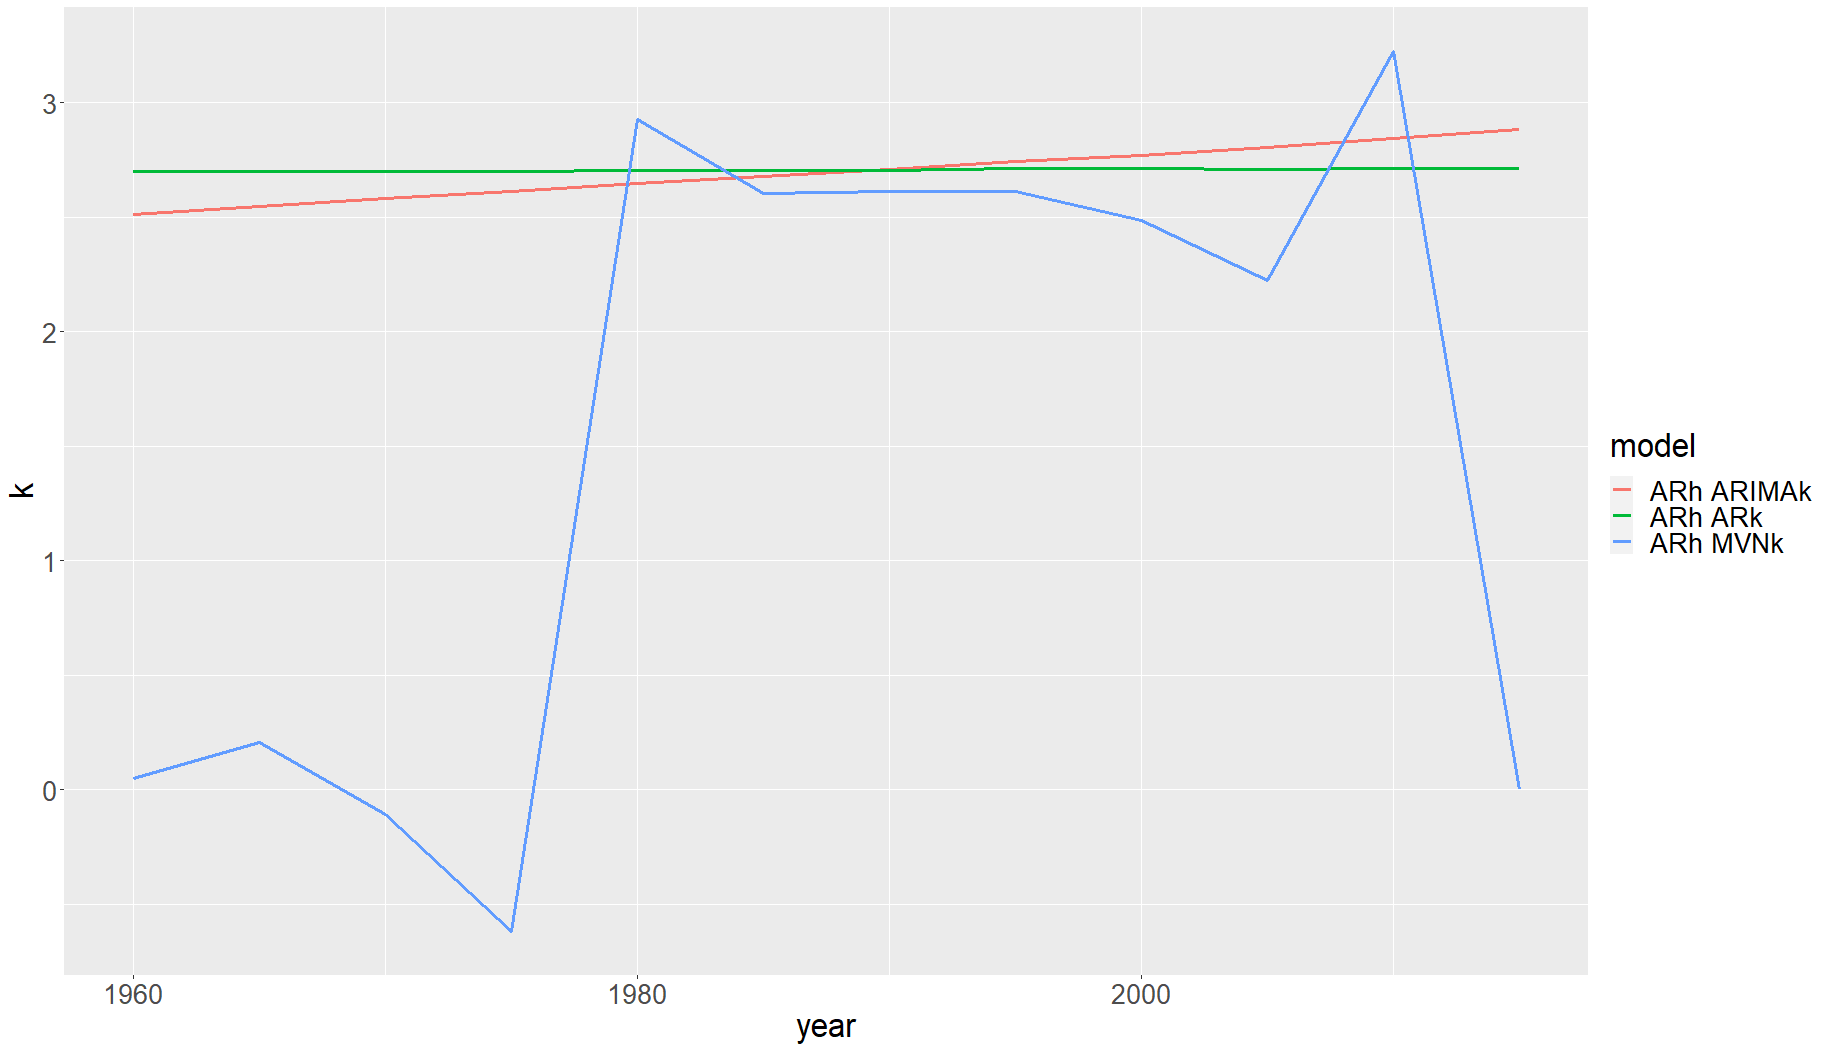
\includegraphics[width = \linewidth]{Burkina Faso/5/k.jpg}
\caption{Estimated $k$}
\end{figure}

\newpage
\begin{figure}[H]
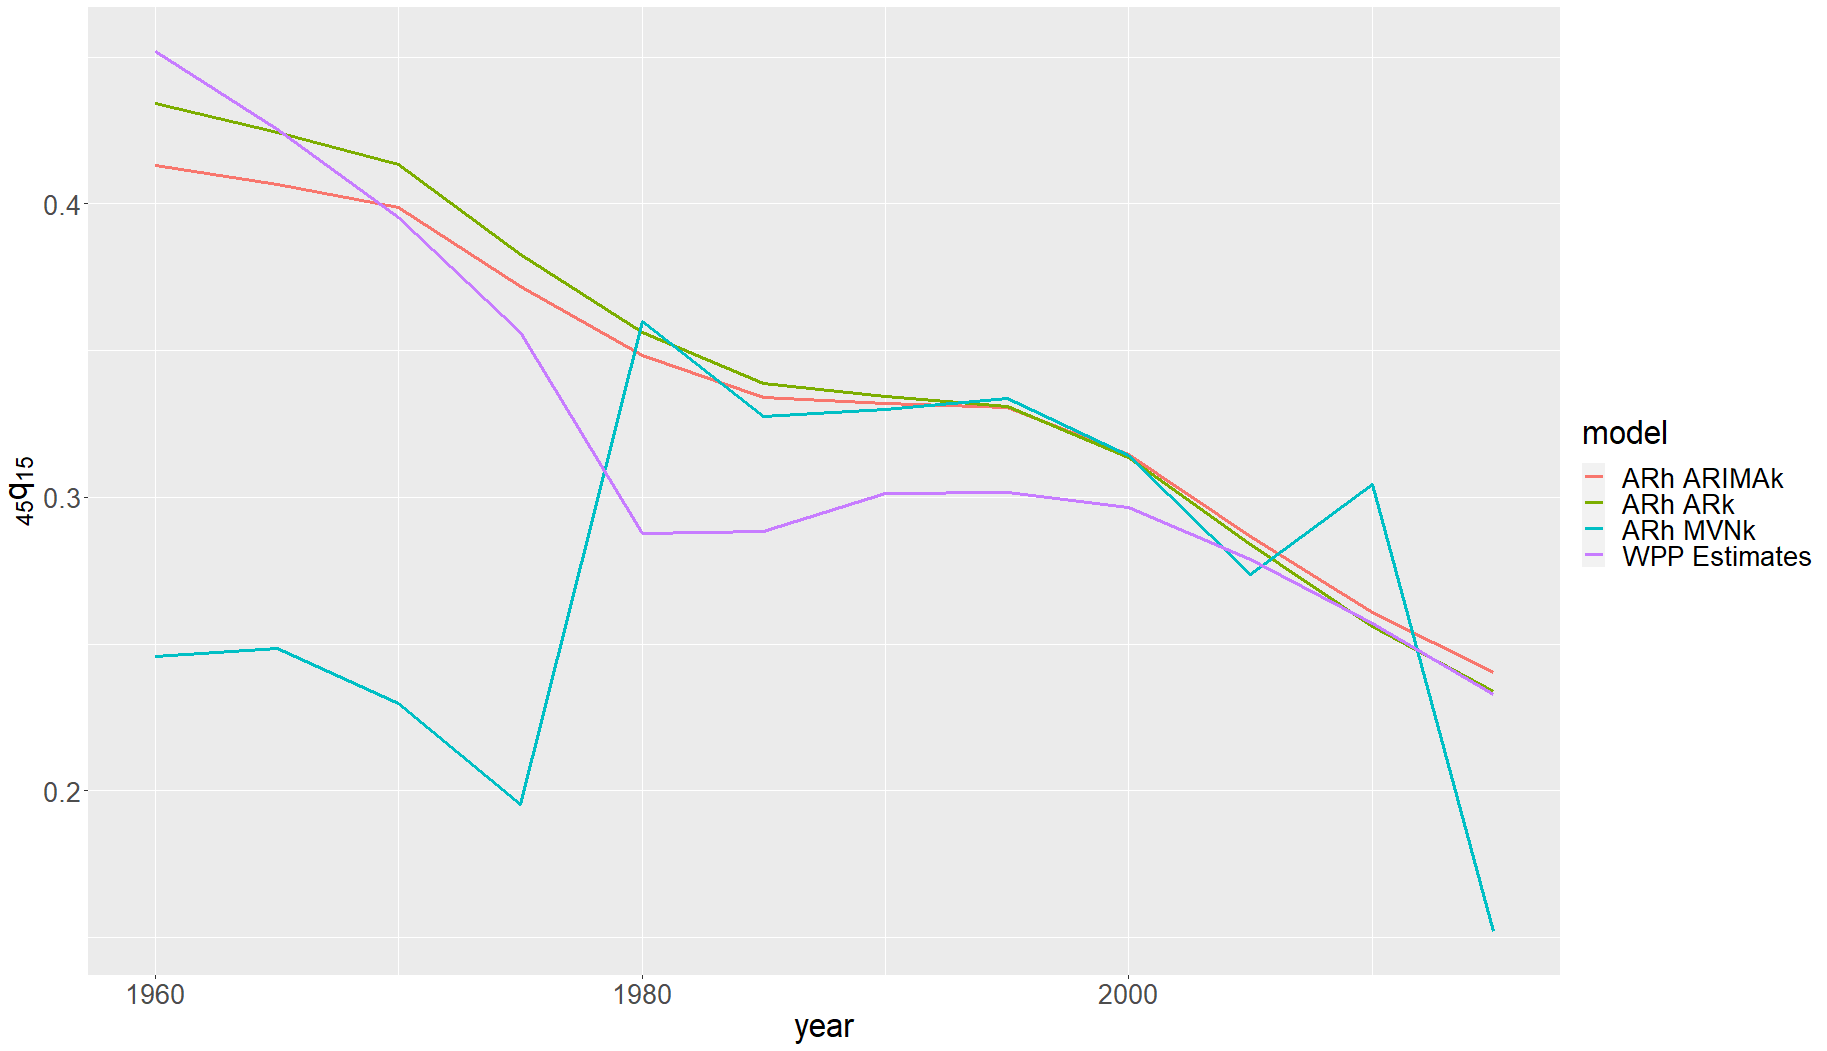
\includegraphics[width = \linewidth]{Burkina Faso/5/45q15.jpg}
\caption{Estimated $_{45}q_{15}$}
\end{figure}
\begin{figure}[H]
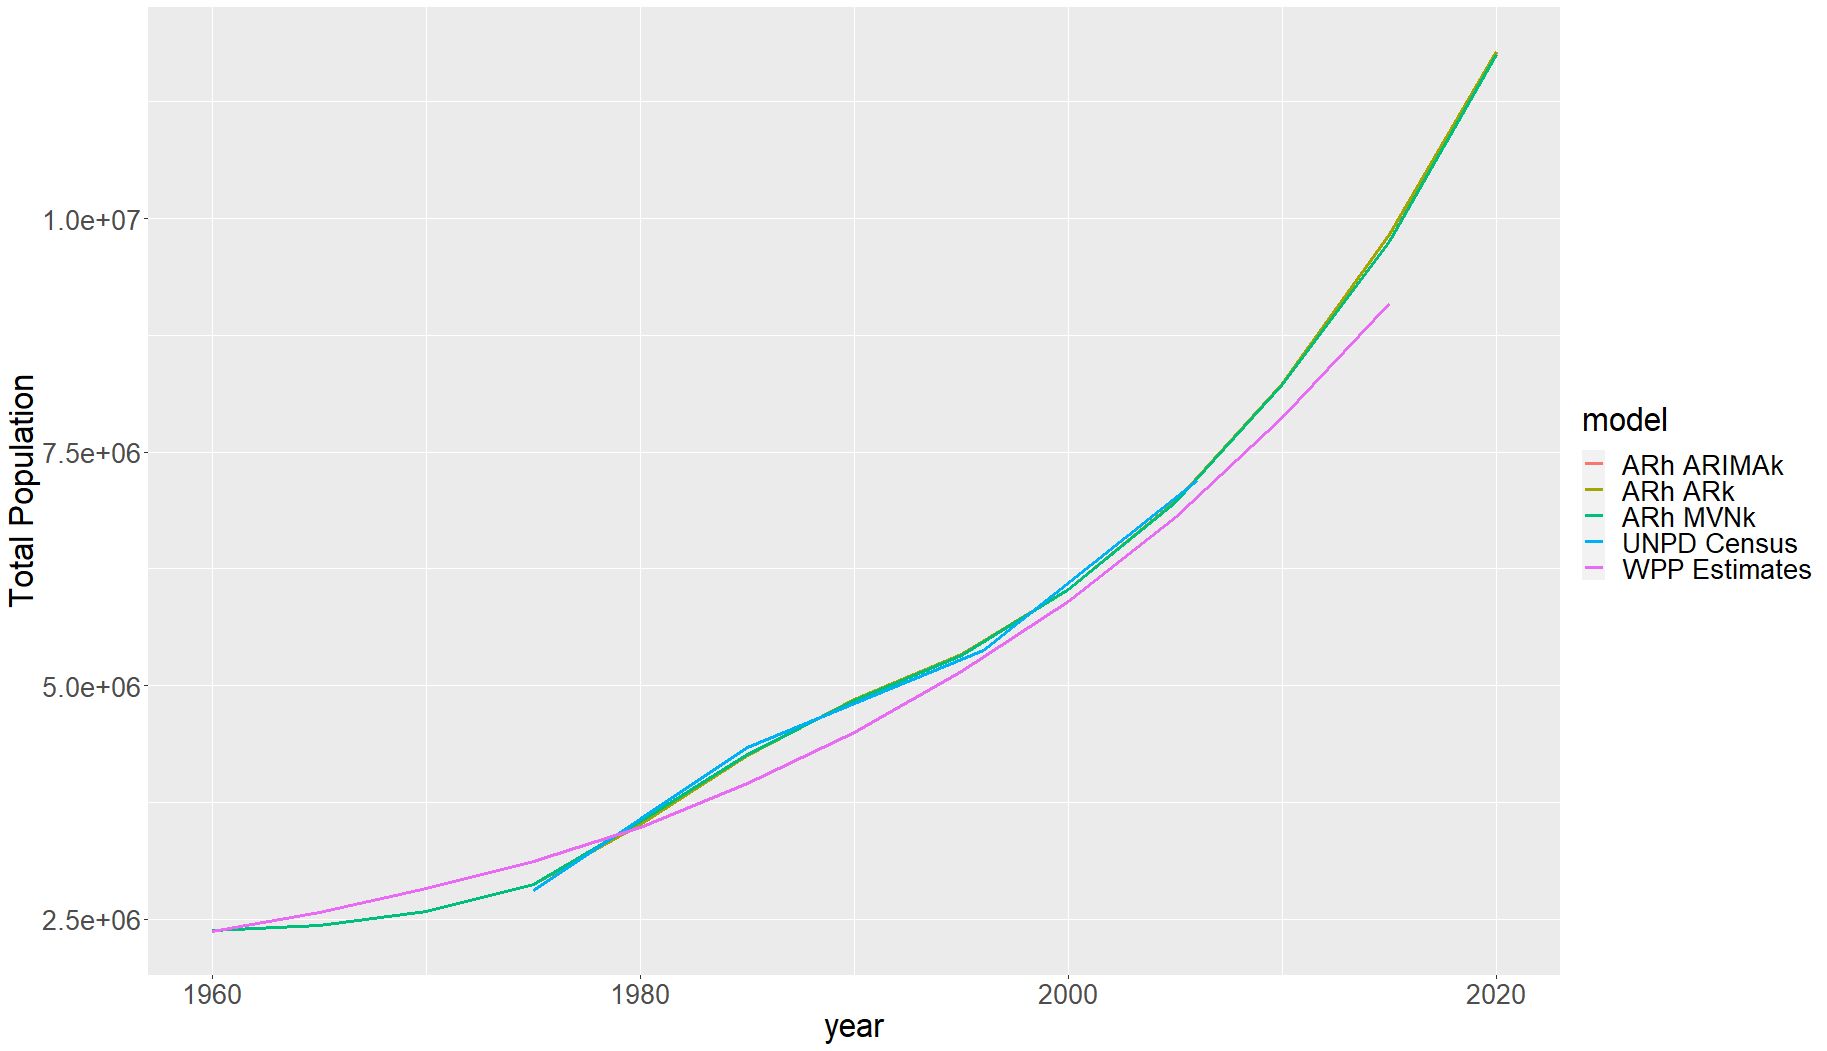
\includegraphics[width = \linewidth]{Burkina Faso/5/total pop.jpg}
\caption{Estimated total population counts}
\end{figure}

\newpage
\begin{figure}[H]
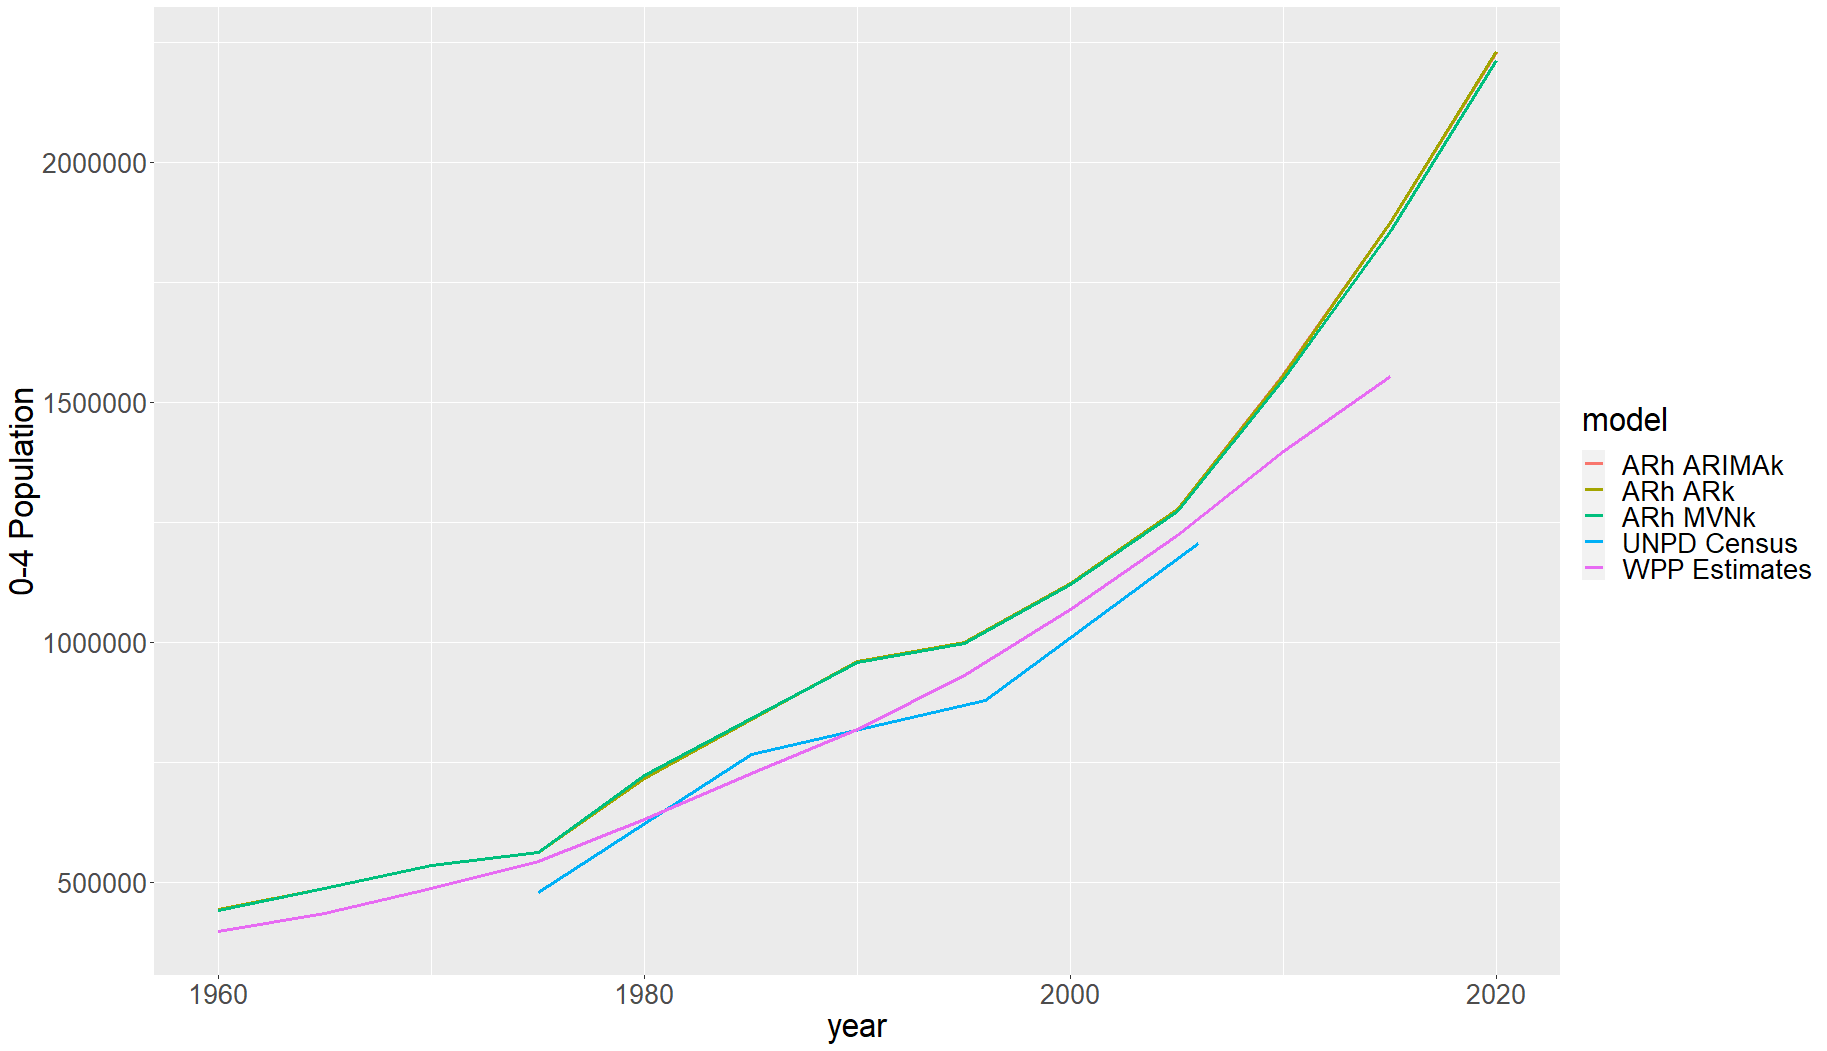
\includegraphics[width = \linewidth]{Burkina Faso/5/0-4 pop.jpg}
\caption{Estimated 0-4 population counts}
\end{figure}
\begin{figure}[H]
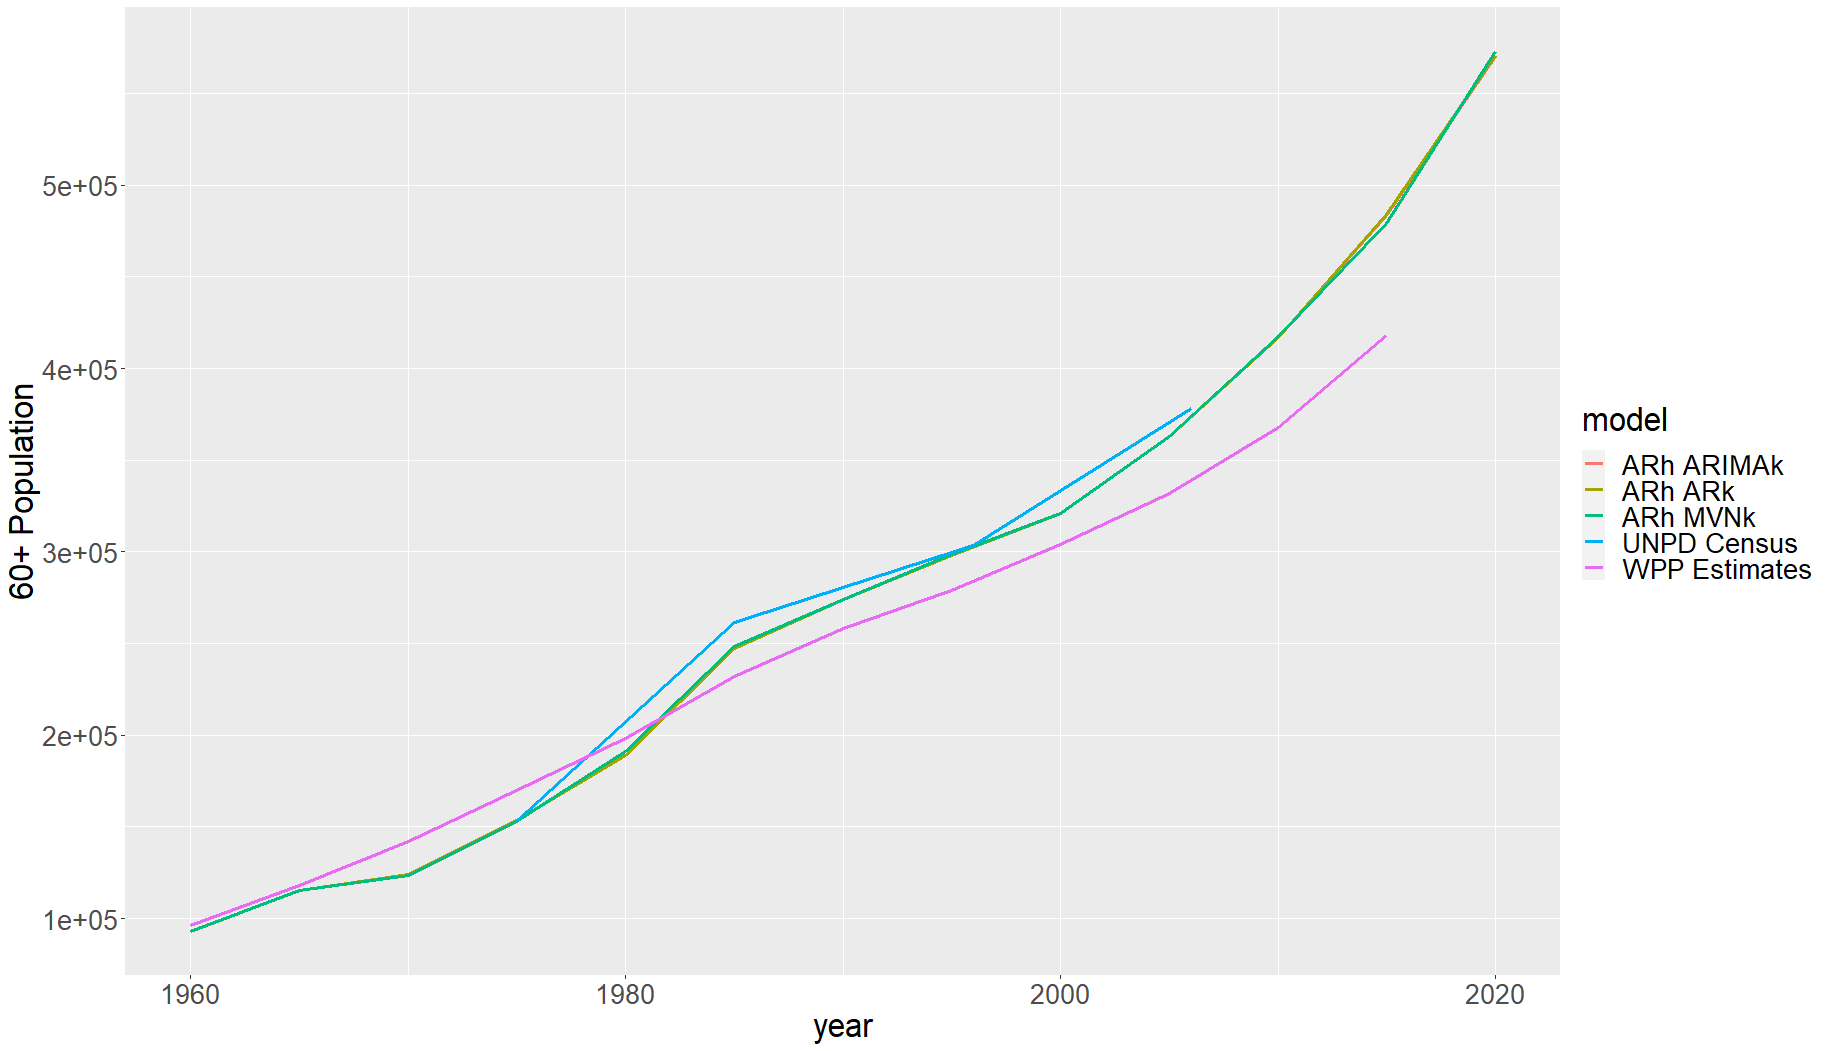
\includegraphics[width = \linewidth]{Burkina Faso/5/60+ pop.jpg}
\caption{Estimated 60+ population counts}
\end{figure}


\newpage
\begin{figure}[H]
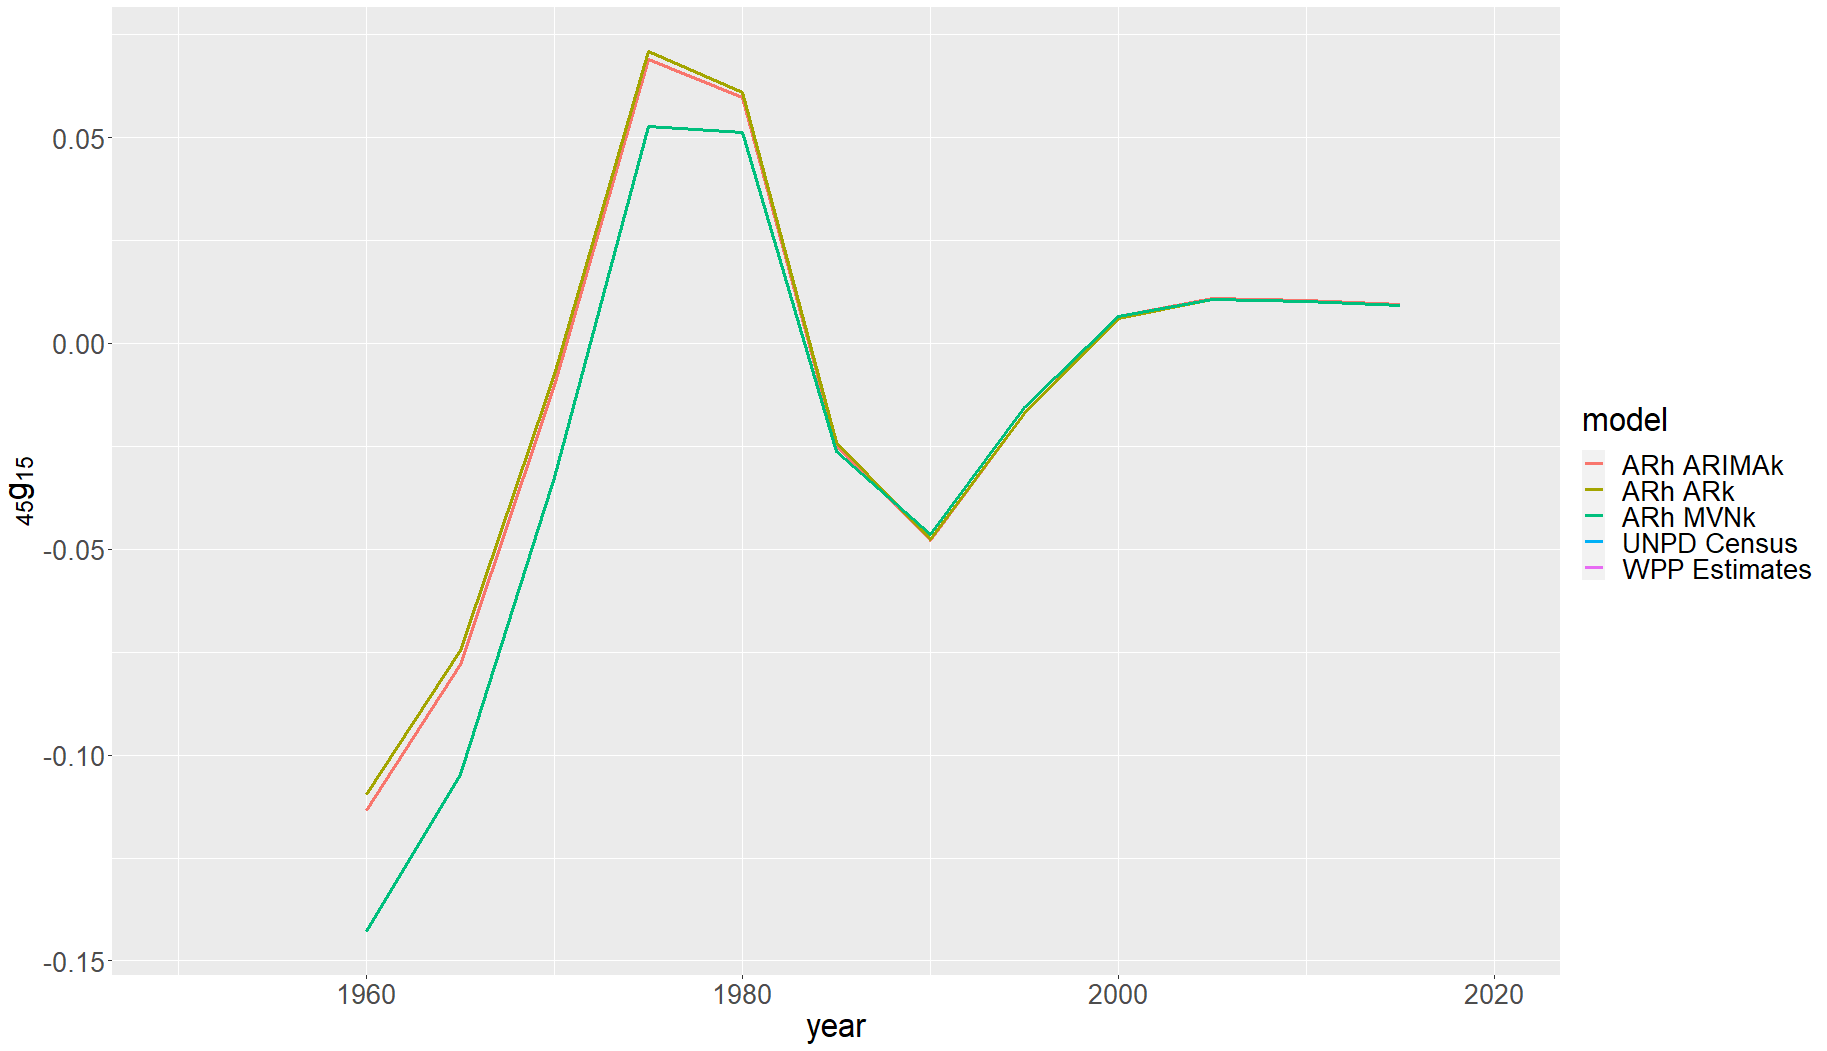
\includegraphics[width = \linewidth]{Burkina Faso/5/15-59 mig.jpg}
\caption{Estimated $_{45}g_{15}$}
\end{figure}
\begin{figure}[H]
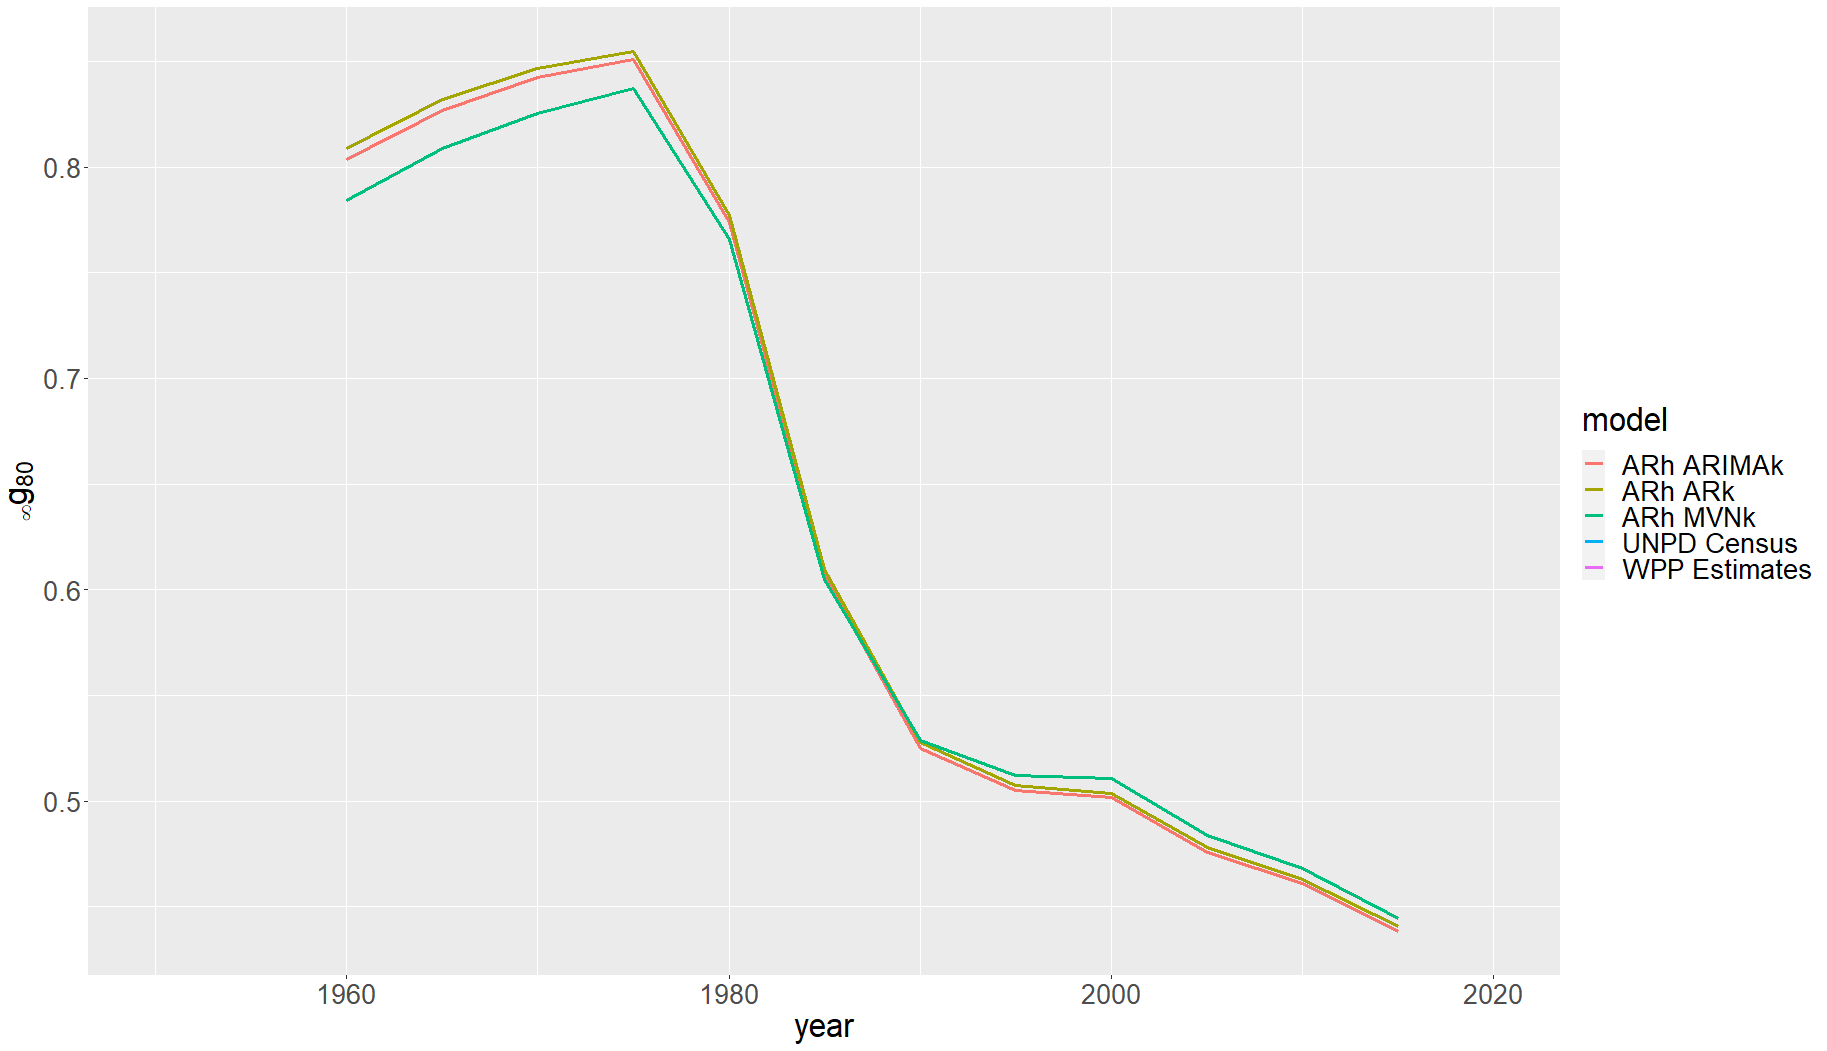
\includegraphics[width = \linewidth]{Burkina Faso/5/80+ mig.jpg}
\caption{Estimated $_{\infty}g_{80}$}
\end{figure}

\newpage
\begin{figure}[H]
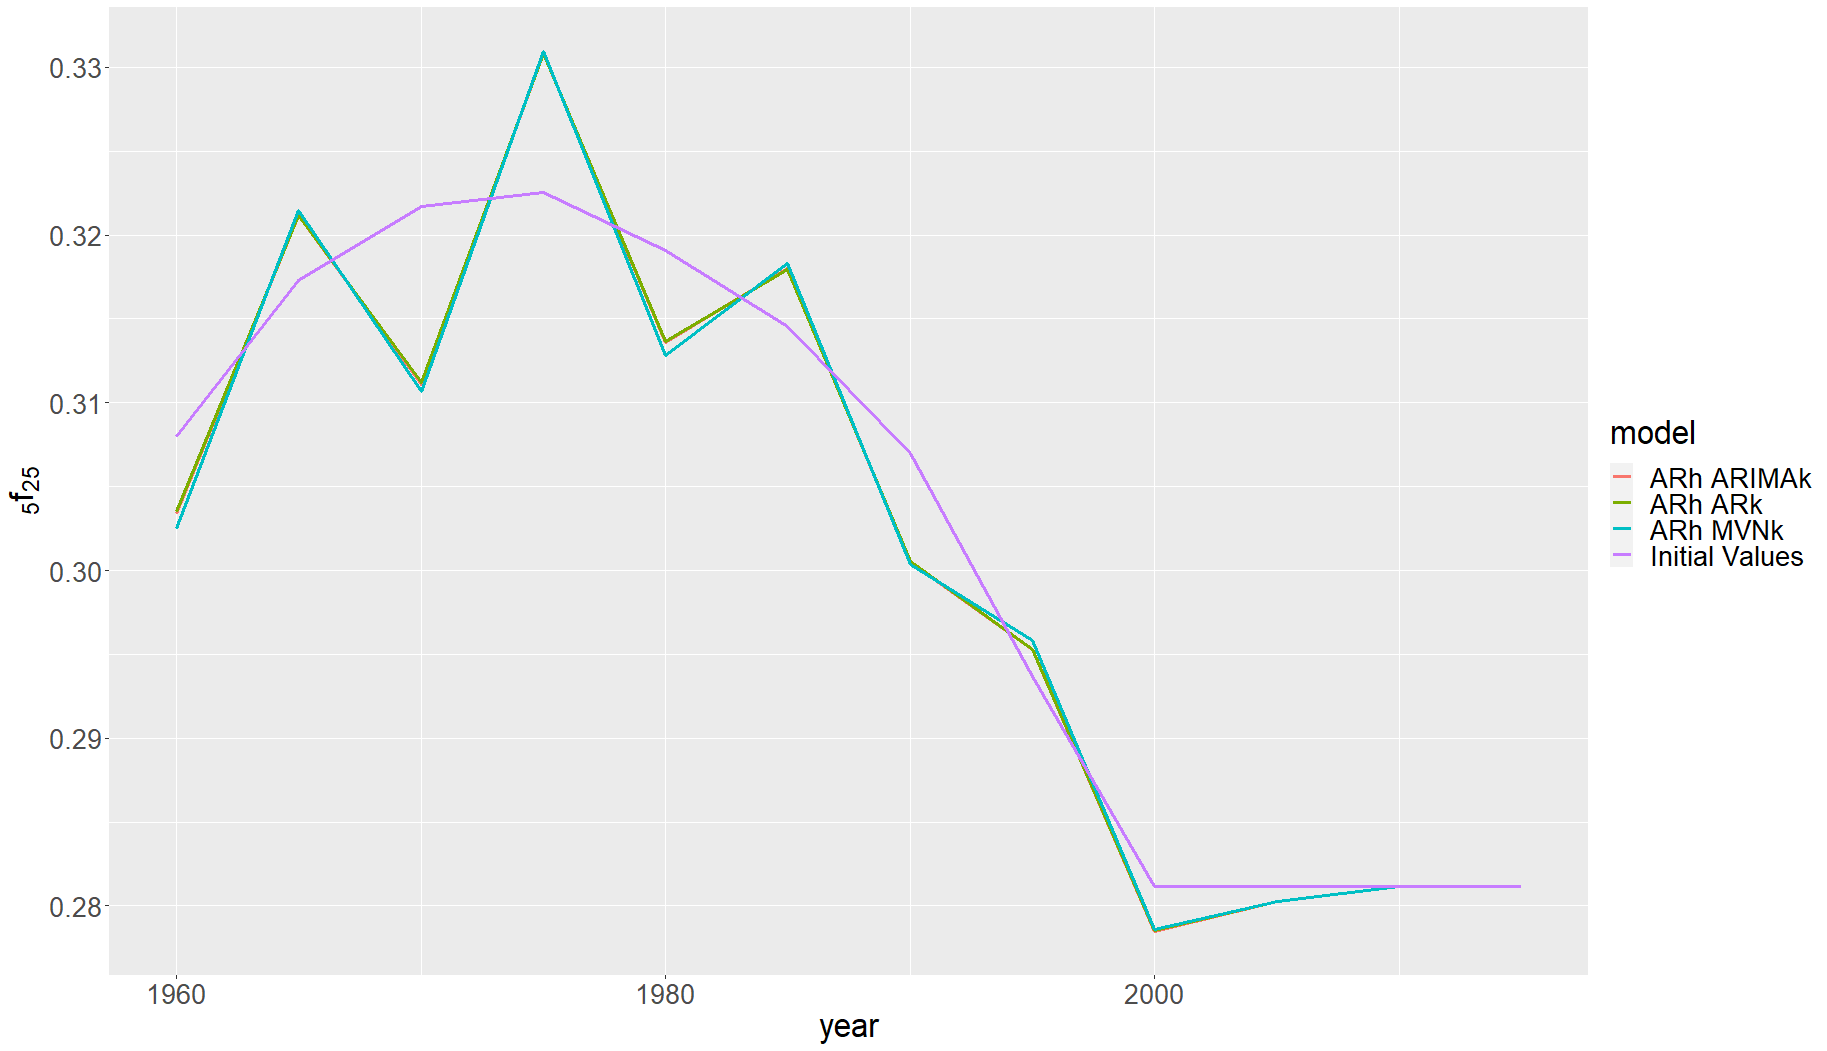
\includegraphics[width = \linewidth]{Burkina Faso/5/25-29 fx.jpg}
\caption{Estimated $_{5}f_{25}$}
\end{figure}



\end{document} 
